\documentclass[../main.tex]{subfiles}

\begin{document}

\subsection{Classical psychophysics and signal detection}

The fundamental objective of psychophysics is to quantify the relationship between the properties of stimuli and the perceived sensation, that is, to find a function $f: \mathbb{R}^k\rightarrow \mathbb{R} $ that maps from stimulus value $x \in \mathbb{R}^k$ to the value of a latent percept. In practice, we are not able to measure the outcome of $f$ directly, and instead measure some indirect consequence of it, such as a response from a participant or a neural signal. This is also known as the \emph{transducer function} \citep{May2013}. Thus, to study psychophysics we must estimate not just $f$ but also some additional function $p(y\mid f(x))$ that maps from the latent percept to the probability of some response $y$. This function is typically stochastic, and motivated by some assumption about the distribution of noise somewhere in the transmission chain from stimulus to decision.

The classical empirical finding, established by Weber and formalized by Fechner \citep{fechner1966elements}, is that the minimal physical difference in stimulus intensities that produces a detectable change in sensation (i.e.\ a JND) is approximately a fractional increment. For example, to perceive the difference in two weight stimuli with 0.75 probability, one weight must be 2\% greater than the other. We can express such a relationship as follows:

\begin{align} \label{eqn:fechner}
\frac{df(x)}{dx} &= \frac{1}{xk},
\end{align}

where $k$ is a scaling constant (the Weber contrast). We can now integrate, giving us $f(x) = \frac{\log(x)}{k} + c$ (though see \citet{Dzhafarov2011} for a more careful derivation). This log-linear transformation is fully specified by determining the two constants, $k$ and $c$.
As noted above, we must also specify a response model for the participants. In the standard setting for discrimination between two intensities $x_1$ and $x_2$, the full response model is the following:
\begin{align}
\tilde{f}(x_1) &= \frac{\log(x_1)}{k} + c + \epsilon_1\\
\tilde{f}(x_2) &= \frac{\log(x_2)}{k} + c + \epsilon_2\\
\epsilon_1, \epsilon_2 &\sim \mathcal{N}(0, \sigma^2),
\end{align}
where $\epsilon_1$ and $\epsilon_2$ are independent Gaussian noise terms. $\tilde{f}(\cdot)$ represents the latent percept, and the subjective response is made by comparing them for the two stimuli:
\begin{align}
p( x_1 > x_2 | \tilde{f}(x_1), \tilde{f}(x_2)) = \Phi\left(\frac{\tilde{f}(x_1)-\tilde{f}(x_2)}{\sqrt{2\sigma}}\right),
\end{align}
where $\Phi(\cdot)$ is the standard normal cumulative distribution function (CDF), also known as the \emph{probit}.
From this, it can also be reasoned that other assumptions about observation noise yield other (non-probit)
transformation of the log-intensity difference. Note that this model is not just a formalization of the
classical Weber-Fechner model, but it is also equivalent to the formulation of the problem under classical
signal detection theory \citep{Green1966}, with the term inside the probit equivalent to $d'$. It can also
be interpreted as the likelihood of the popular diffusion decision model with a fixed response time, the
so-called ``interrogation paradigm" \citep{Bogacz2006}, with the term inside the probit being the
normalized drift rate scaled by time (though neither of these other models has an explicit logarithmic relationship inside the probit).

While the Weber-Fechner law has wide empirical support, especially for moderate values of $x$, such a rigid formulation has some disadvantages. In particular, the log-linear relationship breaks down at very high and low stimulus values where the neural response is either not well-defined or fails to saturate. To address this issue, the standard approach is to independently measure absolute detection and discrimination thresholds, i.e.\ implicitly assume a piecewise linear model with $k_{detection}\ne k_{discrimination}$ \citep[e.g][]{Aguilar1954,Legge1984,Foley1981,Mikkelsen2020}.

Furthermore, it presupposes that the stimulus intensity $x$ is available in the perceptually `correct' units,
i.e.\ ones being presented to the observer's sensors, such that the logarithmic transformation can apply. In practice, this has meant the need to manually search over the space of transformations to correct units, estimate a piecewise linear model with multiple slopes and verify that they are all of similar value, or both. While this is less of a concern for low-level visual and auditory stimuli where the intensity dimension is well-understood, it is of greater relevance to more complex intensity dimensions such as gloss \citep{Chadwick2015}, transparency \citep{Beck1984}, or roughness \citep{BergmannTiest2007}, where finding the units over which the log-linear relationship holds is nontrivial.

Next, the globally linear shape of the function means that estimates of the slope (or JND) in the middle of the intensity domain is highly sensitive to outlier values at the edges of the domain, such as those caused by lapses and guesses on the part of the subject. As a consequence, special care is typically taken to model those empirical phenomena \citep{Prins2012,Wichmann2001,Linares2016}.

Finally, this model is one-dimensional, and does not make predictions of multidimensional stimuli except if they can be transformed to a one-dimensional intensity variable that can be transformed to $d'$. This has meant that practitioners interested in multidimensional psychometric fields can either estimate independent one-dimensional slices through the psychometric field, or write explicit parametric models for detection or discrimination thresholds $k(z)$ as a function of additional contextual variables $z$ \citep[e.g.][]{Watson2017}.

\subsection{Standard empirical methods in context of the standard model}
We now revisit standard experimental methods in context of the above formalization. In the classical approach, whether responses are collected by the methods of constant stimuli or limits, the latent perceptual value is never estimated. Instead, each stimulus pair is repeated many times, such that average accuracies can be estimated. Then, a psychometric function in probability space can be fit directly to these probabilities, and the various thresholds estimated from it. In the case of heuristic staircases such as PEST \citep{Taylor1967}, the threshold is read out from the final step of the staircase. In parametric model-based methods such as QUEST \citep{Watson1983}, the threshold can be estimated from the model used. In both cases, the fact that the standard Weber-Fechner model does not simultaneously apply at sub- and supra-threshold levels means that while a psychometric function can be fit to staircase data, it would not provide good estimates of the psychometric slope or JND.

\subsection{Towards nonparametric psychophysics}

We return the Weber-Fechner formulation (Eq.~\ref{eqn:fechner}), to reflect on the desiderata for a more general nonparametric psychophysics: what is the minimal set of assumptions that one should make about the relationship between external stimulus and internal percept? We argue that the primary requirement is for the relationship to be monotonic in the intensity dimension, i.e.\ for increases in external stimulus to drive increases (or zero change) in the internal percept. Formally this gives the following generalized Fechnarian law:
\begin{align}
\frac{df}{dx} &= g(x),
\end{align}
where $g: \mathbb{R} \rightarrow \mathbb{R}^+$, though in practice we operate with the psychometric transfer function
$f(x)$ directly.
For a multidimensional stimulus $x \in \mathbb{R}^k$, this generalized law applies to the partial derivative with respect to the stimulus intensity dimension, and not necessarily other dimensions that describe properties of the stimulus with respect to which perception may be nonmonotonic.

We take as our model of $f(x)$ a Gaussian process (GP) prior. A GP is a stochastic process that defines a distribution over functions (in our case, psychometric fields) $p(f(x))$, such that the distribution of any finite set of values measured from these functions (in our case, the psychometric field evaluated at a set of points) is jointly multivariate normal.

A GP is described by two functions, a prior mean function $\mu_{\theta}(x)$ and a kernel function $K_{\theta}(x, x')$ that defines the covariance in function values for any pair of points in the parameter space: $\textrm{Cov}[f(x_1), f(x_2)] = K_{\theta}(x_1, x_2)$. The kernel is typically constructed so that the covariance between function values is high when $x_1$ and $x_2$ are close, and low when $x_1$ and $x_2$ are far apart, which induces smoothness in the function across the parameter space: similar stimuli will produce similar outcomes, whereas disparate stimuli will not affect each other. With a GP, the posterior for the function values at any collection of points will be a multivariate normal whose mean and covariance can be written in closed form (and will in general depend on the covariance function and prior mean). As with other kernel-based methods such as kernel density estimation, appropriate choices of these two functions can yield priors that prefer simpler models when data are limited while still converging to any true function in the limit of data. It is also straightforward for the mean and kernel functions to operate over multidimensional inputs (this is, in fact, the standard setting for GPs), making this generalization both multidimensional and potentially nonlinear. See \citet{rasmussen2006gaussian} for a full review of GPs.

The observation model remains the same as in the classical setting, with the assumption of Gaussian noise giving way to a probit transformation. Alternate transformations such as the logit or Weibull CDF are also possible, but unnecessary if the underlying underlying psychometric model is flexible enough, as a GP is. GPs perform a local interpolation such that estimates in the middle of the intensity domain are less sensitive to values at the edges than a global linear model, making them more robust to guesses and lapses. This formulation thus addresses the theoretical concerns raised above: an $f(x)$ modeled by a GP is flexible enough to model correct saturating behavior at high and low intensities, can model incorrect scaling of stimulus intensity, and is multi-dimensional by default.

A closely related approach was given by \citet{Song2018} and \citet{Browder2019}, who also model the psychometric function using a GP. Browder and colleagues consider the general case where both $x_1$ and $x_2$ are allowed to vary, whereas Song and colleagues restrict one of the stimuli (e.g.\ $x_2$, without loss of generality) to be a constant psychophysical standard. We follow the latter, which makes the latent intensity of the standard $f(x_2)$ a constant and reduces the model to a GP classification model over the value of the remaining stimulus. To respect the monotonicity assumption on $f$ in the intensity dimension, Song and colleagues use a linear kernel in that dimension, with an added radial basis function (RBF) kernel in the context dimensions. This provides a multidimensional model with flexibility on contextual effects but does not address scaling and nonlinearity issues in the intensity dimension, and assumes that the effect of contextual dimensions is additive.

In contrast, we use an RBF kernel on all dimensions, using a constraint on the derivatives of the GP to maintain monotonicity in the intensity dimension \citep{Riihimaki2010}. This allows us to consider more flexible psychometric functions both in the intensity dimension and in how the intensity dimension interacts with remaining dimensions. We additionally introduce a new acquisition function for adaptive psychophysics, as discussed below.

\subsection{Extracting slopes and thresholds from multidimensional nonparametric models}
After estimation of the latent psychometric function $f(x)$, there are two possible definitions of a JND or
discrimination threshold. The first takes the formal definition above literally, and defines it as the derivative of the psychometric field at a point $g(x) := f'(x)$. A second definition takes a discretized view, which is that the JND is the change in $x$ needed to increase $f(x)$ by one standard deviation, that is, the smallest stimulus increment $D(x)$ such that $x$ and $x+ D(x)$ can be distinguished with probability at least $\Phi^{-1}(x)$. Alternatively, this can be formulated as $f(x+ D(x))  \ge f(x)+ 1$. The definitions coincide for a linear model of $f(\cdot)$, and JND under either definition can be extracted from the model-estimated $f(\cdot)$ in the nonparametric setting. This can be done by finite-differencing in the case of the derivative definition, or locally-linear interpolation for the step-JND.

\subsection{Gaussian processes with monotonicity information}
To restrict our model to be monotonic in the intensity dimension, we follow \citet{Riihimaki2010} in exploiting the fact that the derivative of a GP is itself a GP. This means that the joint distribution of any set of observations from $f(x)$ and $f'(x)$ is a multivariate normal distribution with closed form mean and covariance. We produce a monotonic prior for $f(x)$ by conditioning on a restriction that $f'(\tilde{x}) \geq 0$, at a set of derivative inducing points $\tilde{x}$. In doing so, we make no assumption about the shape of $f(x)$ other than that its derivative is non-negative, and we are thus able to directly encode the generalized Fechnarian law above. Fig. \ref{fig:prior_samps_fig} gives an illustration of prior samples from this model, along with those from prior work that were described above (the linear-additive kernel, and a full RBF kernel). The prior samples show clearly the restrictiveness of the linear kernel and the unrealistic non-monotonic functions produced by a full RBF kernel. Our monotonic GP is able to encode known monotonicity without sacrificing important flexibility in understanding the relationship between the stimulus and context variables.

\begin{figure}[htb]
    \centering
    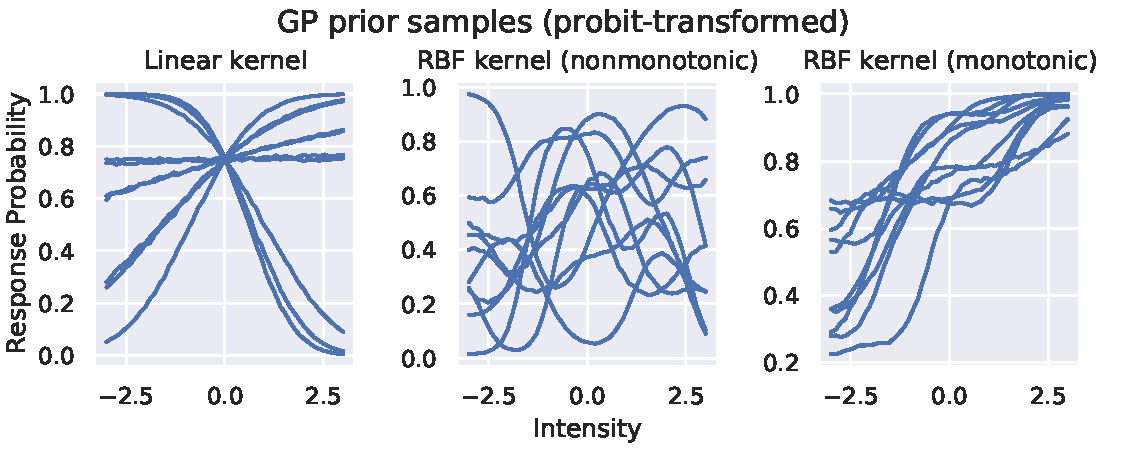
\includegraphics[width=\columnwidth]{prior_samps.pdf}
    \caption{\textbf{Prior samples from the three GP models (in 1d).} \emph{Left:} the linear-additive model's prior is fairly restrictive, but also includes negative slopes (though these are quickly discarded from the posterior after a handful of observations). The additive context (not shown) in $f$-space turns into a shift in probability space, but the posterior slope is restricted to be the same over all contexts. \emph{Middle:} the conventional RBF model is very flexible, including functions that are far from monotonic. \emph{Right:} the approximately-monotonic RBF model is more flexible than the linear kernel model, but excludes the nonmonotonic functions from the prior seen in the other two models. }
    \label{fig:prior_samps_fig}
\end{figure}

\subsection{Inference and acquisition}

A significant advantage of using models for estimating the psychometric function is that it enables active learning and adaptive sampling, which can greatly improve sample efficiency and reduce the time needed to run an experiment. Fig.~\ref{fig:flow_chart_fig} provides an illustration of the active learning process as it can be applied to a psychophysics experiment. We first estimate a model of the data so far (the \emph{inference} step), then use that model to optimize an acquisition function that is maximized at the stimulus parameters we should evaluate next (the \emph{acquisition} step), present the stimulus to the participant and then log the data so we can update the model, and the cycle continues. We now describe these steps in detail.

\begin{figure}[htb]
    \centering
    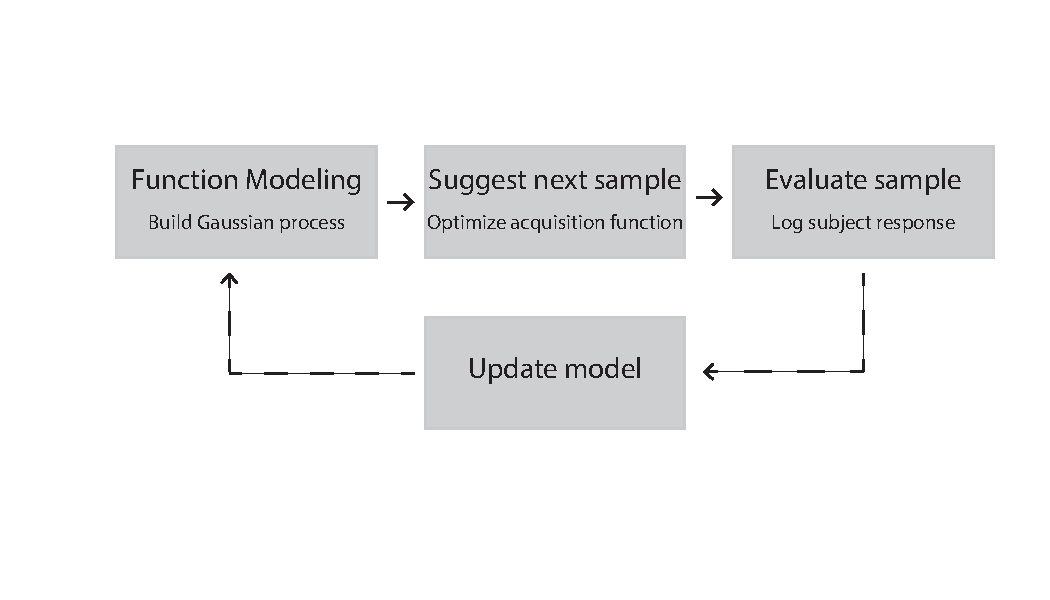
\includegraphics[width=\columnwidth]{flow_chart}
    \caption{\textbf{The active sampling loop.} In our method, the experiment proceeds by first modeling the data using a Gaussian process, optimizing an acquisition function to determine the next stimulus to sample, presenting the stimulus to the participant and collecting the response, and then incorporating that new data into the model to continue the process.}
    \label{fig:flow_chart_fig}
\end{figure}

\subsubsection{Inference}

Our need to update the model frequently, with the human in the loop, means that both model inference and selection of the next point must take a few seconds at most. This precludes the use of full MCMC inference, and requires the use of techniques for scalable approximate GP inference. The standard approach to scalable inference for GPs with non-Gaussian observations such as ours is variational inference \citep[e.g.][]{rasmussen2006gaussian}. Variational inference approximates the posterior distribution $p(f\mid y)$ with a simpler distribution $q(f\mid y)$ (often a multivariate normal), chosen to minimize the Kullback-Leibler (KL) divergence between the true and approximate posteriors. This is made tractable by minimizing an objective known as the evidence lower bound (ELBO), and is much faster than performing full MCMC inference (for more on variational inference, see \cite{Blei2017}). However, variational inference is difficult to implement with monotonicity information because the approximate posterior $q(f\mid y)$ needs to be monotonic, which can render the ELBO intractable.
Consequently, previous approaches to monotonic GPs used expectation propagation \citep{Riihimaki2010}.


Rather than implement custom inference methods for the various models we consider, to maximize simplicity and scalability we use conventional variational inference throughout. In the monotonic case, we do this by performing conventional, non-monotonic inference, and then performing rejection sampling on the non-monotonic posterior to construct an approximately monotonic posterior: we draw a large set of samples from the GP, and attempt to exclude all samples with negative derivative values.
To avoid long delays we draw a fixed number of samples, in which case rejection sampling does not guarantee that we will achieve the desired number of monotonic posterior samples. In that case, we draw the samples that least violate the monotonicity constraint by including those samples with negative derivatives that are closest to 0. This produces a posterior that is nearly monotonic, and as the variational posterior converges with increasing data, the rejection rate in the sampling goes to zero assuming the data-generating function is indeed monotonic.
\subsubsection{Acquisition}
\begin{figure*}[htb]
    \centering
    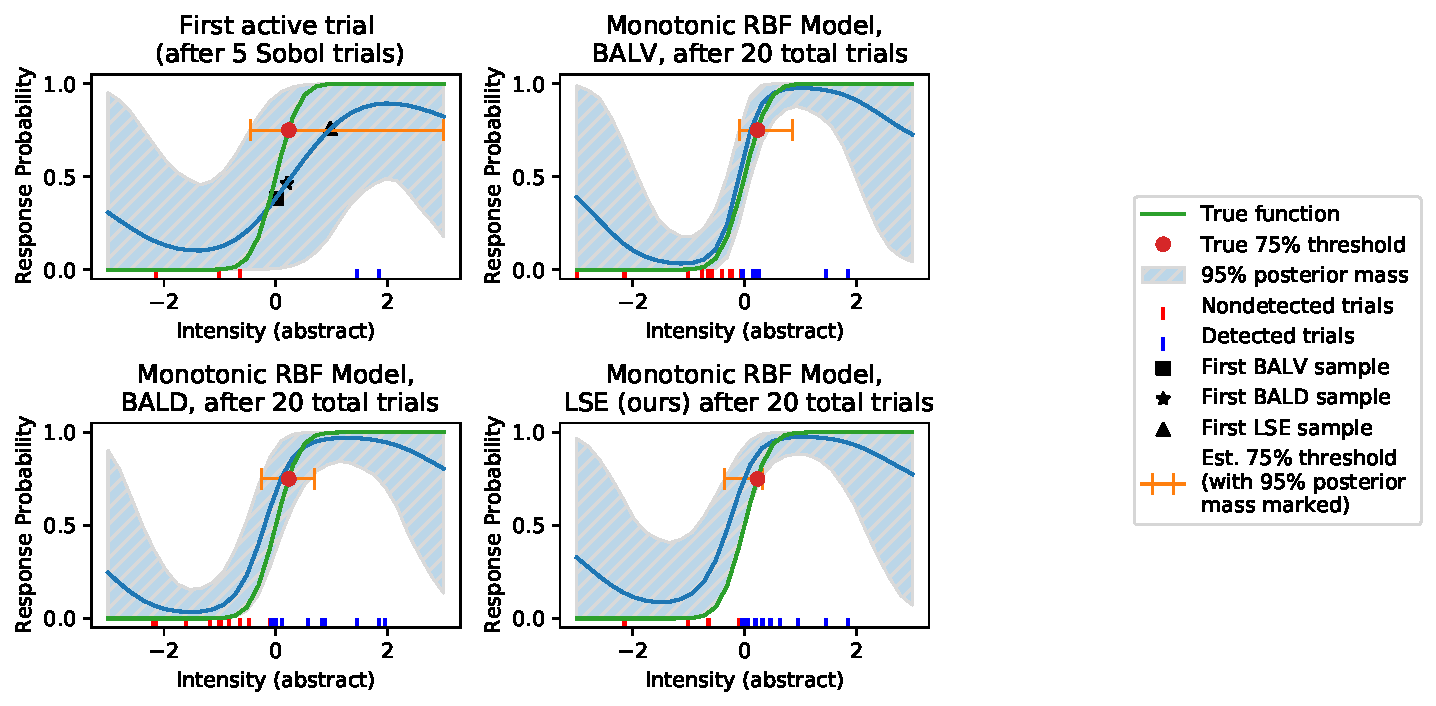
\includegraphics[width=\textwidth]{same_model_different_acq.pdf}
    \caption{\textbf{Different acquisition functions can target different experimenter objectives.} \emph{Top left}: The posterior over a simple linear psychometric function after 5 Sobol trials, and the first adaptive trial selected under BALD, BALV, and LSE targeting the 75\% threshold. LSE samples where the current estimate would place the threshold, whereas BALD and BALV both sample close to 0.5, where uncertainty is maximized and the most information about the function can be gained. \emph{Top right, bottom left, and bottom right}: The same estimates after 15 additional adaptive trials, showing that while BALV and BALD sample across different values of the function and therefore provide a better estimate of it overall, LSE samples near the eventual threshold, achieveing a tighter final interval. The monotonic RBF model is used for all three acquisition functions.}
    \label{fig:same-model-different-acq}
\end{figure*}


Our primary purpose in inserting a model into the experimentation process is to use active learning to reduce the number of observations required to determine the psychophysical quantities of interest. The two ingredients of such an active learning process are the model (the GP just described), and a policy that determines how to choose the next stimulus to present based on the current model estimates.
Conventionally in GP active learning, such a policy is encoded in an \emph{acquisition function} $a(x)$ that maps from the stimulus parameters to the desirability of sampling in that location. By choosing different acquisition functions, it is possible to make the active learning process reflect different goals, for example estimating the JND vs.\ estimating the detection threshold (see Fig.~\ref{fig:same-model-different-acq} for an illustration of this point). The next point can be selected by choosing the point where the acquisition function is maximized, or selected randomly in proportion to the value of the acquisition function (the latter being an instance of Thompson sampling; \cite{Thompson1933}). Using Thompson sampling instead of solving the minimization problem on $a(x)$ can provide speed benefits, as well as encourage model exploration. A final baseline strategy is to use a random or quasi-random sequence over the search domain. In practice, we begin the experiment with a fixed number of trials drawn from a quasi-random sequence (in our case, a Sobol sequence; \cite{Sobol1967}), after which we sample points according to our acquisition function. We consider three acquisition functions below: mutual-information maximization (also known as Bayesian Active Learning by Disagreement or BALD; \cite{Houlsby2011}), posterior variance minimization (also known as Bayesian Active Learning by Variance or BALV; \cite{Settles2009}), and level set estimation (LSE; \cite{Gotovos2013}). Note that while BALD and BALV have been used in psychometrics previously, the introduction of LSE is new, and is motivated by the problem of threshold estimation. We discuss all three acquisition functions next.

\paragraph{Bayesian active learning by variance (BALV)}
If the objective is to estimate the full psychometric function, one natural solution is to simply attempt to minimize the uncertainty over the whole psychometric surface, by sampling wherever the current posterior variance is highest. This strategy has been previously used for estimation of psychometric fields and thresholds \citep{Song2018,Song2017b,Gardner2015a,Schlittenlacher2018,Schlittenlacher2020}. The probit transformation means that even if variance is very high in some parts of the space, that variance cannot be reduced if the response probability there is squashed to 0 or 1. Thus, BALV is conventionally performed with respect to the variance of the response distribution, i.e.\ $Bernoulli(\Phi(f(x))):=\Phi(f(x))(1-\Phi(f(x)))$. If uncertainty over $f(x)$ is uniform over $x$, BALV reduces to sampling wherever the probability of response is closest to 0.5 (though in practice sampling is slightly more variable due to variations in the variance of $f(x)$). This is somewhat undesirable if one is interested not in the 0.5-threshold, but in another threshold such as 0.75. It is also greedy: repeatedly sampling at the point of highest current uncertainty is not equivalent to sampling at points which will maximally reduce total, global uncertainty.

\paragraph{Bayesian active learning by disagreement (BALD)}
Related to the issue brought up above, minimizing the uncertainty over the full surface may be better accomplished by sampling a point which will most reduce the posterior entropy, in expectation over outcomes. This acquisition function is known as BALD in the GP literature \citep[e.g.][]{Houlsby2011}, and is equivalent to the mutual information between the unseen outcome $y$  and the response probability $\Phi(f(x))$. In the psychophysics literature it is among the most common acquisition functions, used in both nonparametric models (\emph{Ibid.}) and more classical adaptive methods \citep[e.g.][]{Watson2017,Kontsevich1999,Brand2002,DiMattina2015,Hall1981,Watson1983,Kujala2006,Lesmes2010}. BALD is less greedy than BALV (using effectively one-step lookahead) and is more likely to sample over the full domain of the function. While this may be desirable for estimating the full psychometric surface or the JND, this is less desirable when the experiment objective is to target a specific part of the surface.

\paragraph{Level Set Estimation (LSE)}
When the goal of an experiment is threshold estimation, we would ideally want to focus sampling at the places that most improve our estimate of the threshold. When the function is monotonic with respect to stimulus intensity, the detection threshold is a point in one dimension, forms a line in 2d, a plane in 3d, and so on. Formally, it is called a \emph{level set} of $f(x)$, and is the set of all points $x$ such that $f(x)=T$ for some desired threshold level $T$. Our goal in psychophysical threshold estimation is to identify the threshold stimulus intensity for any given value of the contextual variables, which corresponds to identifying the entire level set across the parameter space.

\citet{Gotovos2013} proposed an acquisition function for level-set estimation, called the LSE acquisition function, that selects points according to their ambiguity of being either above or below threshold. This provides a natural approach for active sampling to reduce uncertainty in the threshold intensity. They show how the ambiguity measure can easily be computed directly from the posterior mean and variance of $f(x)$, though in contrast to this prior work we use $\Phi(f(x))$ instead, which gives markedly better performance in our setting. To select the next stimulus to display, we use standard gradient optimization techniques to optimize the LSE acquisition function and identify the maximum ambiguity point.

We also develop and explore a novel Thompson-sampling variant of LSE (LSETS) which, instead of optimizing the acquisition function, takes a large, joint sample from the GP posterior on a space-filling design and selects the next stimulus $x$ according to its probability of its $f(x)$ being closest to $T$. This improves running time by avoiding solving an optimization problem for each sample selection.

\end{document}
